\subsection*{c. La clienta Lena Cacioppo compró un producto de cada subcategoría de Furniture. Deberás elegir los productos que desees e indicar como parte de esta consulta, la información que se agregará en cada caso.}

Primero seleccionamos los productos de la categoría Furniture y los agrupamos por subcategoría, eligiendo en cada una el producto con el id más alto, para obtener un producto por subcategoría. Renombramos este resultado como muebles.\\ \\
Usando una proyección, agregamos a cada producto los datos fijos de la compra: el id de la clienta Lena Cacioppo (\textit{LC-16870}), el id de la orden (\textit{US-2026-169552}), la fecha del pedido (30 de octubre de 2026), la fecha de envío (29 de noviembre de 2026), el modo de envío (\textit{Second Class}) y la cantidad (1).

Expresión:
\[
\begin{aligned}
&\pi_{\text{'LC-16870'} \to cliente,\; pid,\; \text{'US-2026-169552'} \to orden,\; \text{DATE('2026-10-29')} \to pedidoen,} \\
&\quad{}_{\text{DATE('2026-11-29')} \to enviadoen,\; \text{'Second Class'} \to modoenvio,\; 1 \to cantidad}\Bigg( \\
&\qquad \rho_{muebles}\Big( \qquad\qquad \pi_{pid} \\
&\hspace{2.2 cm}\qquad\qquad \gamma_{subcategory;\; \mathrm{MAX}(productid) \to pid} \\
&\hspace{2.2 cm} \qquad\qquad \sigma_{category = \text{'Furniture'}}\; products \qquad\Big)\Bigg)\\
\end{aligned}
\]
Resultados obtenidos:

\begin{figure}[h!]
\centering
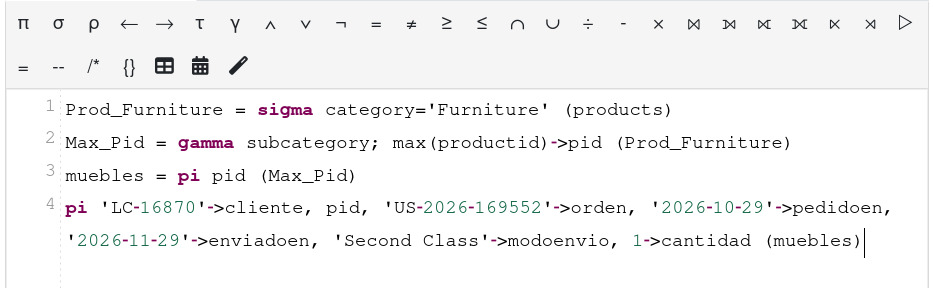
\includegraphics[width=0.9\textwidth]{imagenes/3c(1).png}
\caption{Consulta}
\end{figure}

\begin{figure}[h!]
\centering
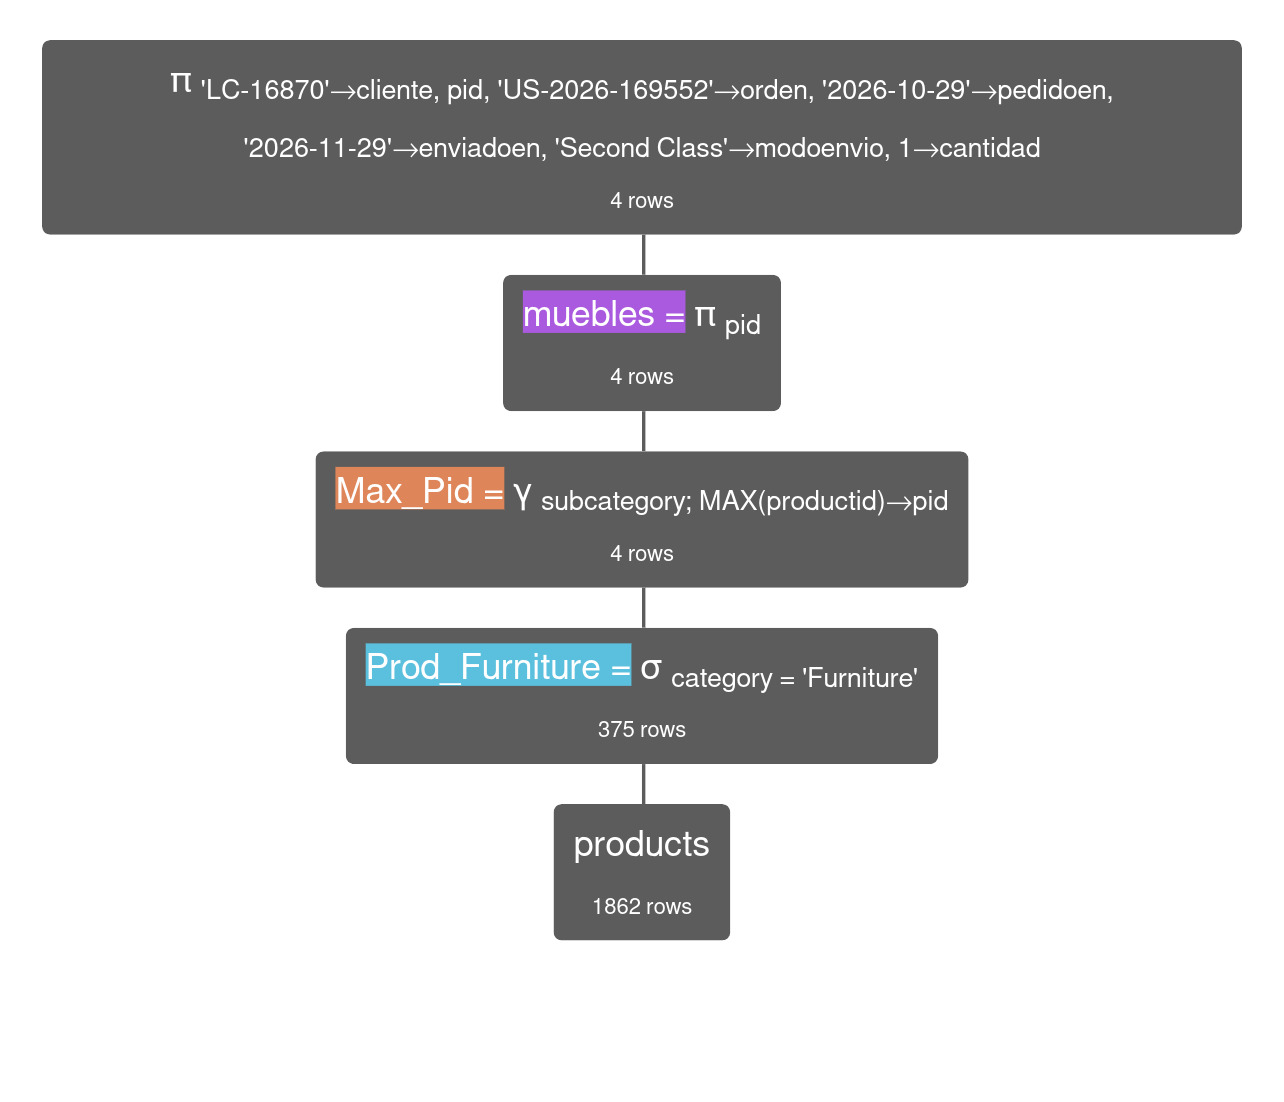
\includegraphics[width=0.72\textwidth]{imagenes/3c(2).png}
\caption{Árbol de consulta.}
\end{figure}

\begin{figure}[h!]
\centering
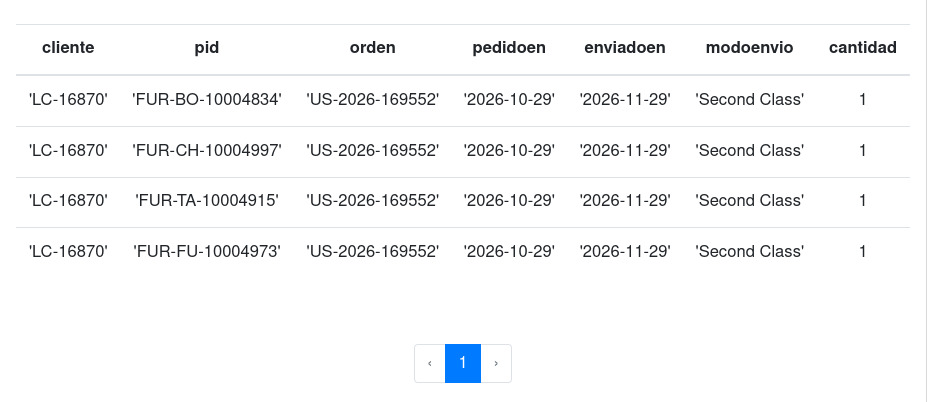
\includegraphics[width=0.8\textwidth]{imagenes/3c(3).png}
\caption{Resultado de consulta.}
\end{figure}
